\section{General Probability Theory}

\subsection{\texorpdfstring{$\sigma$}{sigma}-algebra}

\begin{definition}
\leavevmode
\begin{itemize}
    \item The set of all possible outcomes of an experiment is called the \textbf{state space}, denoted by $\Omega$.
    \item The family of all possible subsets of $\Omega$, i.e.\ the power set is denoted by $2^\Omega$.
\end{itemize}
\end{definition}

\begin{definition}[$\sigma$-algebra]
A family of subsets $\A \subset 2^\Omega$ is called a $\sigma$-algebra if it satisfies
\begin{enumerate}[(i)]
    \item $\Omega \in \A$, or $\emptyset \in \A$.
    \item Closure under complement: If $A \in \A$ then $A^c \in \A$.
    \item Closure under countable unions and intersections: If a sequence of sets $(A_i)_{i \geq 1}$ belongs to $\A$, then $\bigcup_{i=1}^{\infty} A_i$ (or $\bigcap_{i=1}^{\infty} A_i$, by De Morgan's law\footnote{$\bigcap_{i=1}^{\infty} A_i = \left(\bigcup_{i=1}^{\infty} A_i^c\right)^c$.}) also belongs to $\A$.
\end{enumerate}
The smallest possible $\sigma$-algebra is the trivial $\sigma$-algebra: $\{\emptyset, \Omega\}$. The largest possible $\sigma$-algebra is $2^\Omega$. Between the two, we have e.g.\ for a 6-faced dice, $\A = \{\{1\}, \{2, 3, 4, 5, 6\}, \emptyset, \Omega\}$.
\end{definition}

\begin{definition}[$\sigma$-algebra generated by families of sets]
\leavevmode
\begin{itemize}
    \item Let $\mathcal{C}$ be an arbitrary family of subsets of $\Omega$. We denote by $\sigma(\mathcal{C})$ the smallest $\sigma$-algebra which contains every set in $\mathcal{C}$ (i.e.\ $\mathcal{C} \subseteq \sigma(\mathcal{C})$) and call this the $\sigma$-algebra generated by $\mathcal{C}$.

    \item (Borel $\sigma$-algebra) An important example is the Borel $\sigma$-algebra over any topological space $\Omega$, denoted by $\B(\Omega)$, which is the $\sigma$-algebra generated by the open sets of $\Omega$ (or, equivalently, by the closed sets\footnote{To show this, we just need to show that $\sigma(\mathcal{C}) \subseteq \B(\Omega)$ and $\B(\Omega) \subseteq \sigma(\mathcal{C})$. All closed sets are complements of open sets. Since $\B(\Omega)$ being a $\sigma$-algebra is closed under complement, it contains all the closed sets, i.e.\ $\mathcal{C} \subseteq \B(\Omega) \Rightarrow \sigma(\mathcal{C}) \subseteq \B(\Omega)$. A similar argument can be used to show that $\mathcal{O} \subseteq \sigma(\mathcal{C}) \Rightarrow \B(\Omega) = \sigma(\mathcal{O}) \subseteq \sigma(\mathcal{C})$.}). In other words, $\B(\Omega) := \sigma(\mathcal{O}(\Omega))$, where $\mathcal{O}(\cdot)$ denotes the collection of all open sets.
    \begin{itemize}
        \item Recall that an open set of $\R$ is a subset $E \subseteq \R$ such that for every $x \in E$ there exists $\epsilon > 0$ such that $B_\epsilon(x) = \{y \in \R : |x - y| < \epsilon\}$ is contained in $E$.
        \item A set $F \subseteq \R$ is said to be closed if $F^c$ is open.
        \item $\R$ and $\emptyset$ are simultaneously both open and closed sets.
    \end{itemize}

    \item ($\sigma$-algebra generated by a random variable) Given $X : (\Omega, \A) \to (\Psi, \G)$, the $\sigma$-algebra generated by $X$, denoted $\sigma(X)$ is the smallest $\sigma$-algebra on $\Omega$ such that $X$ is a random variable, that is, $X$ is measurable with respect to $\sigma(X)$ and $\G$. Equivalently, $\sigma(X) = X^{-1}(\G) = \{X^{-1}(S) \mid S \in \G\}$ (by Definition~1.3.1 and Theorem~1.3.2).
\end{itemize}
\end{definition}

\begin{theorem}
The Borel $\sigma$-algebra $\B(\R)$ is generated by intervals of the form $(-\infty, a]$ where $a \in \mathbb{Q}$ is a rational number.
\end{theorem}

\begin{proof}
Let $\mathcal{O}$ denote the collection of all open intervals. Since every open set in $\R$ is an at most countable union of (disjoint) open intervals, we have $\sigma(\mathcal{O}) = \B(\R)$.

Let $\mathcal{D}$ be the collection of all intervals of the form $(-\infty, a]$, $a \in \mathbb{Q}$. For any $a < b$, $a, b \in \mathbb{Q}$,
\[
(a, b) = \bigcup_{n=1}^{\infty} (a, b - \tfrac{1}{n}] = \bigcup_{n=1}^{\infty} (-\infty, b - \tfrac{1}{n}] \cap (-\infty, a]^c,
\]
which implies that $(a, b) \in \sigma(\mathcal{D})$, i.e.\ $\mathcal{O} \subseteq \sigma(\mathcal{D}) \Rightarrow \sigma(\mathcal{O}) \subseteq \sigma(\mathcal{D})$. However, every element of $\mathcal{D}$ is a closed set (complement of an open set) so $\mathcal{D} \subseteq \B(\R) \Rightarrow \sigma(\mathcal{D}) \subseteq \B(\R) = \sigma(\mathcal{O})$, completing the proof.
\end{proof}

\subsection{Probability Space}

\begin{definition}[measurability]
\leavevmode
\begin{itemize}
    \item Given a state space $\Omega$ and a $\sigma$-algebra $\A \subseteq 2^\Omega$, the duple $(\Omega, \A)$ called a \textbf{measurable space}.
    \item A subset $A \in \Omega$ is said to be $\A$-measurable if $A \in \A$. We call $A$ an \textbf{event}.
\end{itemize}
\end{definition}

\begin{definition}[probability measure]
Let $\Omega$ be a nonempty set, and let $\A$ be a $\sigma$-algebra of subsets of $\Omega$. A probability measure $\P$ is a function that, to every set $A \in \A$, assigns a number in $[0, 1]$. We require:
\begin{enumerate}[(i)]
    \item $\P(\Omega) = 1$.
    \item (countable additivity) whenever $A_1, A_2, \cdots$ is a countable sequence of disjoint sets in $\A$, then
    \[
    \P\left(\bigcup_{i=1}^{\infty} A_i\right) = \sum_{i=1}^{\infty} \P(A_i).
    \]
\end{enumerate}
The triple $(\Omega, \A, \P)$ is called a \textbf{probability space}.
\end{definition}

\begin{theorem}[probability measure $\P$ is continuous along monotone sequences of events]
If $\P : \A \to [0, 1]$ is a probability measure, then
\begin{itemize}
    \item If $(A_i)_{i \geq 1} \in \A$ is increasing, i.e.\ $A_1 \subseteq A_2 \subseteq A_3 \subseteq \cdots$ with $\lim_{i \to \infty} A_i = \bigcup_{i=1}^{\infty} A_i = A$, denoted $A_i \uparrow A$, then
    \[
    \lim_{i \to \infty} \P(A_i) = \P\left(\lim_{i \to \infty} A_i\right) = \P(A).
    \]
    \item If $(A_i)_{i \geq 1} \in \A$ is decreasing, i.e.\ $A_1 \supseteq A_2 \supseteq A_3 \supseteq \cdots$ with $\lim_{i \to \infty} A_i = \bigcap_{i=1}^{\infty} A_i = A$, denoted $A_i \downarrow A$, then
    \[
    \lim_{i \to \infty} \P(A_i) = \P\left(\lim_{i \to \infty} A_i\right) = \P(A).
    \]
\end{itemize}
\end{theorem}

Proof omitted (course notes pp.8--9).

\subsection{Random Variables}

Let $(\Omega, \A)$ and $(\Psi, \G)$ be two measurable spaces (Definition~1.2.1).

\begin{definition}[measurability of a function]
A function $X : \Omega \to \Psi$ is said to be \textbf{measurable} with respect to $\A$ and $\G$ if the pre-image $X^{-1}(G) = \{\omega : X(\omega) \in G\} \in \A$ for all $G \in \G$, or equivalently, $X^{-1}(\G) \subseteq \A$.
\end{definition}

\begin{definition}[random variable]
A \textbf{random variable} is a real-valued function $X : \Omega \to \R$ that is measurable with respect to $\A$ and $\B(\R)$. That is, the pre-image $X^{-1}(B) = \{\omega : X(\omega) \in B\} \in \A$ for all Borel sets $B \in \B(\R)$. We sometimes simply say $X$ is $\A$-measurable.
\end{definition}

\begin{definition}[almost sure equality of two r.v.s]
Two random variables $X$ and $Y$ are said to be \textbf{equal almost surely}, written $X \overset{\text{a.s.}}{=} Y$ if the set $\{\omega : X(\omega) \neq Y(\omega)\}$ is of probability zero.
\end{definition}

The theorem below says, to check if a function is measurable w.r.t.\ a $\sigma$-algebra, it suffices to check the pre-image of the generating family of the $\sigma$-algebra.

\begin{theorem}[measurability of a function]
Let $\mathcal{C}$ be a class of subsets of $\Psi$ such that $\sigma(\mathcal{C}) = \G$. In order for a function $X : \Omega \to \Psi$ to be measurable with respect to $\A$ and $\G$, it is necessary and sufficient that $X^{-1}(\mathcal{C}) \subseteq \A$.
\end{theorem}

\begin{proof}
By Definition~1.3.1, we just need to show that $X^{-1}(\mathcal{C}) \subseteq \A$ iff $X^{-1}(\sigma(\mathcal{C})) \subseteq \A$.

The backward direction is straightforward since $\mathcal{C} \subseteq \sigma(\mathcal{C})$. To show the forward direction, suppose $X^{-1}(\mathcal{C}) \subseteq \A$. Define
\[
\mathcal{K} = \{B \in \sigma(\mathcal{C}) \mid X^{-1}(B) \in \A\}.
\]
It is easy to verify that $\mathcal{K}$ is a $\sigma$-algebra (by using results on pre-image of complement, union, and intersection). By assumption, $\mathcal{C} \subseteq \mathcal{K}$ and therefore $\sigma(\mathcal{C}) \subseteq \mathcal{K}$. The definition of $\mathcal{K}$ then implies $X^{-1}(\sigma(\mathcal{C})) \subseteq \A$.
\end{proof}

\begin{corollary}
(from Theorem~1.3.1 and Theorem~1.1.1) A function $X : \Omega \to \R$ is a random variable if and only if $\{\omega : X(\omega) \leq a\} = X^{-1}((-\infty, a]) \in \A$ for all $a \in \mathbb{Q}$.
\end{corollary}

\textit{Example to Corollary~1.3.1.} Consider the probability space $([0, 1], \B[0, 1], \P)$ where $\P$ is the Lebesgue measure, i.e.\ $\P[a, b] = b - a$, $0 \leq a \leq b \leq 1$. Consider the identity function, i.e.\ $X(\omega) = \omega$. To show $X$ is a r.v., just note that
\[
X^{-1}((-\infty, a]) = \{\omega : X(\omega) \leq a\} = [0, a] \in \B[0, 1],
\]
for all $a \in \mathbb{Q}$, $a \leq 1$.

\begin{corollary}
(from Theorem~1.3.1) Two random variables $X$ and $Y$ are independent iff $\P(X \leq a, Y \leq b) = \P(X \leq a)\P(Y \leq b)$ for all $a, b \in \mathbb{Q}$.
\end{corollary}

\begin{theorem}[pre-image of $\sigma$-algebra on domain is also $\sigma$-algebra]
Let $X : \Omega \to \Psi$ be a mapping. Let $\G$ be a $\sigma$-algebra on $\Psi$. Then $X^{-1}(\G)$ is a $\sigma$-algebra on $\Omega$.
\end{theorem}

\begin{proof}
We verify the axioms for a $\sigma$-algebra:
\begin{enumerate}[(i)]
    \item $X^{-1}(\Psi) = \Omega \Rightarrow \Omega \in X^{-1}(\G)$ as $\Psi \in \G$.
    \item Let $S \in X^{-1}(\G)$. Then $S = X^{-1}(G)$ for some $G \in \G$. We know that the pre-image of set difference equals the set difference of the respective pre-images, so
    \[
    \Omega \setminus S = X^{-1}(\Psi) \setminus X^{-1}(G) = X^{-1}(\underbrace{\Psi \setminus G}_{\in \G}) \Rightarrow \Omega \setminus S \in X^{-1}(\G).
    \]
    \item Let $(S_i)_{i \geq 1} \in X^{-1}(\G)$. Then $S_i = X^{-1}(G_i)$ for some $G_i \in \G$ for all $i$. It follows that
    \[
    \bigcup_{i=1}^{\infty} S_i = \bigcup_{i=1}^{\infty} X^{-1}(G_i) = X^{-1}\left(\bigcup_{i=1}^{\infty} G_i\right) \in X^{-1}(\G),
    \]
    where we used the fact that the union of pre-images is the same as the pre-image of the union.
\end{enumerate}
\end{proof}

\subsection{Expectation}

\begin{definition}[characteristic function, mgf]
\leavevmode
\begin{itemize}
    \item The \textbf{characteristic function} of a r.v.\ $X$ is given by $\Phi_X(t) = \E[e^{itX}]$.
    \item The \textbf{moment generating function} of a r.v.\ $X$ is given by $M_X(t) = \E[e^{tX}]$.
\end{itemize}
\end{definition}

\begin{definition}[expectation]
Let $X$ be a r.v.\ on a probability space $(\Omega, \A, \P)$. The \textbf{expectation} of $X$ is
\[
\E(X) = \int_\Omega X(\omega) \, d\P(\omega).
\]
When $X$ is a simple random variable, i.e.\ it takes on only finitely many values, it can be written as
\[
X = \sum_{i=1}^{n} x_i \indic_{A_i} \iff X(\omega) = \sum_{i=1}^{n} x_i \indic_{A_i}(\omega), \quad \omega \in \Omega
\]
where $x_i \in \R$ and $A_i = \{\omega : X(\omega) = x_i\} \in \A$. Its expectation is given by
\[
\E(X) = \sum_{i=1}^{n} x_i \P(A_i) = \sum_{i=1}^{n} x_i \P\{X = x_i\}.
\]
\end{definition}

\begin{definition}[$L^1$]
We say $X$ is \textbf{integrable} if $\E(X) < \infty$. The space of integrable r.v.s is denoted by $L^1(\Omega, \P)$.
\end{definition}

\begin{theorem}
The random variable $X$ is integrable if and only if $\E(|X|) < \infty$.
\end{theorem}

\begin{proof}
We can write $X = X^+ - X^-$ where $X^+ = \max(X, 0)$ and $X^- = \max(-X, 0)$. Then $|X| = X^+ + X^-$.
\end{proof}

\begin{theorem}[Jensen's inequality]
Let $g : \R \to \R$ be a convex function and $X$ a r.v.\ with $\E|X| < \infty$. Then
\[
g(\E[X]) \leq \E[g(X)].
\]
\end{theorem}

\subsection{Conditional Expectation}

\subsubsection{Conditional Expectation w.r.t.\ a Partition}

Given a simple random variable $X$ taking values $x_1, \cdots, x_n$,
\[
\mathcal{D}(X) = \{D_1^X, \cdots, D_n^X\} \quad \text{where } D_i^X = \{X = x_i\}
\]
is the partition of $\Omega$ associated with $X$.

\begin{definition}[conditional expectation w.r.t.\ a partition]
For any partition $\mathcal{D} = \{D_1, \cdots, D_n\}$ of $\Omega$, the conditional expectation of a simple random variable $X$ is given by
\[
\E(X|\mathcal{D}) = \sum_{i=1}^{n} \E(X|D_i) \indic_{D_i} = \underbrace{\sum_{i=1}^{n} \sum_{j=1}^{m} x_j \P(D_j^X | D_i) \indic_{D_i}}_{\text{a simple } \sigma(\mathcal{D})\text{-measurable r.v.}},
\]
where $\E(X|D_i) = \E(X \indic_{D_i}) \P(D_i)^{-1}$ is the usual conditional expectation, and $\mathcal{D}(X)$ partitions $\Omega$ w.r.t.\ $X$.

If we have two simple random variables $X$ and $Y$, then
\[
\E(X|Y) := \E[X|\mathcal{D}(Y)] = g(Y)
\]
for some measurable function $g$, which, clearly, is $\sigma(Y)$-measurable.
\end{definition}

\begin{result}
\leavevmode
\begin{itemize}
    \item Given a partition $\mathcal{D}$ of $\Omega$, $\P(A|\mathcal{D}) = \P(A|\sigma(\mathcal{D}))$ for all $A \in \A$. More generally, $\E(X|\mathcal{D}) = \E(X|\sigma(\mathcal{D}))$.
    \item For a simple random variable $X$, $\sigma(X) = \sigma(\mathcal{D}(X))$.
\end{itemize}
\end{result}

\begin{proof}
For (1), $\E(X|\mathcal{D})$ is clearly $\sigma(\mathcal{D})$-measurable. Now from the uniqueness of conditional expectation (Definition~1.5.2), it suffices to check that for all $A \in \sigma(\mathcal{D})$,
\[
\E[\E(X|\mathcal{D}) \indic_A] = \E[\indic_A X].
\]
We can see that this indeed holds as
\begin{align*}
\E[\indic_A X] &= \E[\E[\indic_A X | \mathcal{D}]] && \text{(tower property)} \\
&= \E[\indic_A \E[X|\mathcal{D}]] && \text{(taking out what is known)}.
\end{align*}

For (2), $X$ is $\sigma(\mathcal{D}(X))$-measurable, so $\sigma(X) \subseteq \sigma(\mathcal{D}(X))$. On the other hand, $\mathcal{D}(X) \subseteq \sigma(X) \Rightarrow \sigma(\mathcal{D}(X)) \subseteq \sigma(X)$, hence the equality.
\end{proof}

\subsubsection{General Conditional Expectation}

\begin{definition}[conditional expectation w.r.t.\ a $\sigma$-algebra]
Let $X$ be a integrable random variable on $(\Omega, \A, \P)$. Given a arbitrary sub-$\sigma$-algebra $\G \subseteq \A$, the \textbf{conditional expectation} of $X$ with respect to $\G$, denoted by $\E[X|\G]$, is the unique integrable random variable satisfying the following conditions:
\begin{enumerate}[(i)]
    \item (measurability) $\E[X|\G]$ is $\G$-measurable, i.e.\ $\E[X|\G]^{-1}(\B(\R)) \subseteq \G$ or $\E[X|\G]^{-1}(B) \in \G$ for all $A \in \B(\R)$.
    \item (partial averaging) For any $A \in \G$, we have
    \[
    \E[\indic_A X] = \E[\indic_A \E[X|\G]]
    \]
    or in integral form $\int_A \E[X|\G](\omega) \, d\P(\omega) = \int_A X(\omega) \, d\P(\omega)$.
\end{enumerate}
\end{definition}

For the definition to make sense, we need to prove the existence and uniqueness of conditional expectation.

\begin{theorem}[existence and uniqueness of conditional expectation]
Let $\G$ be a sub-$\sigma$-algebra of $\A$. Then
\begin{enumerate}
    \item (existence) there exists a conditional expectation $\E[X|\G]$ for any $X \in L^1(\Omega, \P)$.
    \item (uniqueness) any two conditional expectations of $X \in L^1(\Omega, \P)$ respective to $\G$ are equal $\P$-a.s.
\end{enumerate}
\end{theorem}

\begin{proof}
\textbf{Existence.} Suppose $X \in L^1(\Omega, \P)$ then $X^\pm \in L^1(\Omega, \P)$. Without loss of generality, we may assume that $X \geq 0$. Define a new probability measure $\Q$ on $(\Omega, \A)$ by setting for any $A \in \A$,
\[
\Q(A) := \frac{\E[\indic_A X]}{\E[X]}
\]
The probability $\Q$ is absolutely continuous with respect to $\P$ on $\A$ (i.e.\ for $A \in \A$, $\P(A) = 0 \Rightarrow \Q(A) = 0$). This implies that $\Q \ll \P$ on $\G \subseteq \A$ (Remark following Definition~7.1.1). Therefore from the Radon--Nikodym Theorem, there exists a positive $\G$-measurable Radon--Nikodym derivative $\eta = d\Q/d\P \in L^1(\Omega, \P)$ such that
\begin{align*}
\E[\indic_A X] &=: \E[X] \Q(A) \\
&= \E[X] \E[\eta \indic_A] \\
&= \E[\E[X] \E[\eta \indic_A] | \G] \\
&= \E[\eta \E[X] \indic_A]
\end{align*}
then $\eta \E[X]$ is a version of the conditional expectation $\E[X|\G]$.

\textbf{Uniqueness.} Suppose $Y$ and $Y'$ are both $\G$-conditional expectation of $X$. Let $G = \{\omega : Y(\omega) > Y'(\omega)\}$ and we assume that $\P(G) > 0$. To this end, we note that
\[
G := \{Y - Y' > 0\} = \bigcup_{n=1}^{\infty} \{Y - Y' > \tfrac{1}{n}\}
\]
\[
G_n := \{Y - Y' > \tfrac{1}{n}\} = \bigcup_{j=1}^{n} \{Y - Y' > \tfrac{1}{j}\}
\]
By Theorem~1.2.1, $G_n \uparrow G \Rightarrow \P(G_n) \uparrow \P(G)$, so there exists $m > 0$ such that $\P(G_m) > 0$.

Since $Y$ and $Y'$ are both $\G$-conditional expectations, we have by (ii) of Definition~1.5.2 that for every $A \in \G$, in particular $G$, we have $\E[\indic_G Y] = \E[\indic_G Y'] \Rightarrow \E[\indic_G (Y - Y')] = 0$. But
\begin{align*}
\E\left[\indic_G (Y - Y')\right] &\geq \E\left[\indic_{G_m} (Y - Y')\right] && (\indic_G \geq \indic_{G_m}) \\
&\geq \frac{1}{m} \P[G_m] > 0 && (\indic_{G_m} = \indic_{\{Y - Y' > 1/m\}})
\end{align*}
This is a contradiction and hence $\P(G) = 0$.
\end{proof}

\subsubsection{Properties of Conditional Expectation}

\begin{result}
\leavevmode
\begin{itemize}
    \item Consider a constant r.v.\ $X = c$, i.e.\ $X(\omega) = c$ for all $\omega \in \Omega$. Then $\sigma(X)$ is the trivial $\sigma$-algebra $\A_0 = \{\emptyset, \Omega\}$.
    \item $\E[\cdot|\A_0] = \E[\cdot]$.
\end{itemize}
\end{result}

\begin{proof}
For (1), the trivial $\sigma$-algebra is obviously the smallest. Further, $X$ is measurable w.r.t.\ $\A_0$ as
\[
X^{-1}(B) = \begin{cases} \emptyset & \text{if } c \notin B \\ \Omega & \text{if } c \in B \end{cases}
\]
for all $B \in \B(\R)$. As $X^{-1}(\B(\R)) \subseteq \A_0$, by definition $\sigma(X) = \A_0$.

For (2), let $X$ be any random variable on $(\Omega, \A, \P)$. The earlier result implies that $\E[X]$ is $\A_0$-measurable. Next, we check that
\[
\begin{cases} \E(\indic_\emptyset X) = \E(\indic_\emptyset \E(X)) = 0 \\ \E(\indic_\Omega X) = \E(\indic_\Omega \E(X)) = \E(X) \end{cases}
\]
That is, $\E[\indic_A X] = \E[\indic_A \E[X]]$ for all $A \in \A_0$. The required equality follows immediately from the uniqueness of conditional expectation.
\end{proof}

\begin{theorem}[conditional expectation]
Let $X$, $Y$ be two integrable random variables on $(\Omega, \A, \P)$, and $\G$, $\mathcal{H}$ be two sub $\sigma$-algebras of $\A$. Then
\begin{enumerate}
    \item \textbf{(taking out what is known)} If $X$ is $\G$-measurable (or equivalently $\sigma(X) \subseteq \G$), then $\E[X|\G] = X$.

    \item \textbf{(linearity)} For $a, b \in \R$, $\E[aX + bY|\G] = a\E[X|\G] + b\E[Y|\G]$.

    \item \textbf{(tower property)} If $\mathcal{H} \subseteq \G$ then
    \[
    \E[\E[X|\G]|\mathcal{H}] = \E[X|\mathcal{H}]
    \]
    in particular, by taking $\mathcal{H} = \{\emptyset, \Omega\}$ to be the trivial $\sigma$-algebra, we have
    \[
    \E[\E[X|\G]] = \E(X).
    \]

    \item If $X$ is independent of $\G$ in the sense that for all $A \in \sigma(X)$ and $B \in \G$ we have $\P(A \cap B) = \P(A)\P(B)$, then
    \[
    \E[X|\G] = \E[X].
    \]

    \item If $X$ is $\G$-measurable and $Y$ is independent of $\G$ then for any Borel function $h : \R^2 \to \R$ we have
    \[
    \E[h(X, Y)|\G] = H(X),
    \]
    where $H : \R \to \R$ is given by the formula $H(x) = \E[h(x, Y)]$. Consider, e.g.\ $X$ represents the present, $Y$ the future and $\G$ the information generated by past events.

    \item \textbf{(conditional Jensen's inequality)} Let $g : \R \to \R$ be a convex function and for any $\sigma$-algebra $\G \subseteq \A$,
    \[
    g(\E[X|\G]) \leq \E[g(X)|\G].
    \]
\end{enumerate}
\end{theorem}

\begin{proof}
(for 5)
\begin{align*}
\E[h(X, Y)|\G] &= \E[h(x, Y)|\G]\big|_{x=X} && \text{(taking out what is known)} \\
&= \E[h(x, Y)]\big|_{x=X} && \text{($Y$ is independent of $\G$)} \\
&=: H(x)\big|_{x=X}
\end{align*}
\end{proof}

\begin{lemma}[Doob's measurability theorem]
Let $X : \Omega \to \Psi$ be a mapping and $(\Psi, \G)$ a measurable space. A function $Y : \Omega \to \R$ is $\sigma(X)$-measurable if and only if there exists a $\G$-measurable function $h : \Psi \to \R$ s.t.\ $Y = h(X)$.
\end{lemma}

\begin{remark}
Doob's measurability theorem tells us for a integrable random variable $Y$, $\E[Y|\sigma(X)]$ which by definition is $\sigma(X)$-measurable, must be a function of $X$.
\end{remark}

\subsubsection{Geometric Interpretation of Conditional Expectation}

\begin{theorem}
Let $X$ be a square integrable random variable, i.e.\ $\E\left[X^2\right] < \infty$. Then $\E[X|\G]$ is the orthogonal projection of $X$ on $L^2(\Omega, \P)$. This means that for every square integrable $\G$-measurable $Z$,
\[
\E\left[(X - Z)^2\right] \geqslant \E\left[(X - \E[X|\G])^2\right]
\]
with equality if and only if $Z = \E[X|\G]$.
\end{theorem}

\begin{remark}
One can show that $X - \E(X|\G)$ is orthogonal to $\E(X|\G)$. That is,
\[
\E\left[(X - \E(X|\G)) \cdot \E(X|\G)\right] = 0.
\]
\end{remark}

\begin{proof}
(Sketch) We consider
\[
\E\left[(X - Z)^2\right] = \E\left[(X - \E(X|\G) + \E(X|\G) - Z)^2\right]
\]
\[
= \E\left[(X - \E(X|\G))^2\right] + \E\left[\hblue{(\E(X|\G) - Z)^2}\right] + 2\underbrace{\E\left[(X - \E(X|\G))(\E(X|\G) - Z)\right]}_{(*)}
\]
But
\begin{align*}
(*) &= \E\left[\E\left[(X - \E(X|\G))(\E(X|\G) - Z) \middle| \G\right]\right] && \text{(tower property)} \\
&= \E\left[(\E(X|\G) - Z) \underbrace{\E\left[(X - \E(X|\G)) \middle| \G\right]}_{= \E(X|\G) - \E(X|\G) = 0}\right] = 0 && \text{(taking out what is known)}
\end{align*}
and therefore $\E\left[(X - Z)^2\right] \geqslant \E\left[(X - \E[X|\G])^2\right]$.
\end{proof}

\subsection{Visual Representation of Expectation}

\[
\E(X) = \int_\Omega X(\omega) \, d\P(\omega)
\]

The lower Riemann sum is pictured below, with $A_k = \{\omega \in \Omega : y_k \leq X(\omega) < y_{k+1}\}$.

\begin{center}
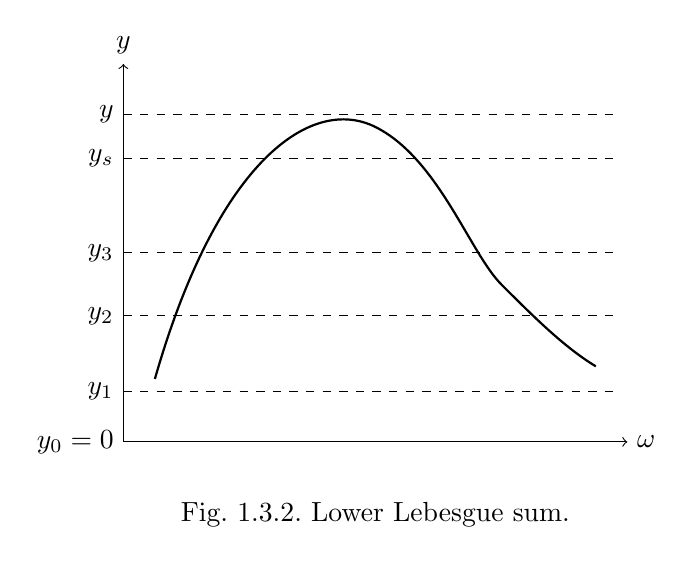
\begin{tikzpicture}[scale=0.8]
    % Axes
    \draw[->] (0,0) -- (8,0) node[right] {$\omega$};
    \draw[->] (0,0) -- (0,6) node[above] {$y$};

    % Curve (representing X(omega))
    \draw[thick] (0.5,1) .. controls (1.5,4.5) and (3,5.5) .. (4,5)
                 .. controls (5,4.5) and (5.5,3) .. (6,2.5)
                 .. controls (6.5,2) and (7,1.5) .. (7.5,1.2);

    % Horizontal dashed lines for y levels
    \draw[dashed] (0,0.8) -- (7.8,0.8);
    \draw[dashed] (0,2) -- (7.8,2);
    \draw[dashed] (0,3) -- (7.8,3);
    \draw[dashed] (0,4.5) -- (7.8,4.5);
    \draw[dashed] (0,5.2) -- (7.8,5.2);

    % Y-axis labels
    \node[left] at (0,0) {$y_0 = 0$};
    \node[left] at (0,0.8) {$y_1$};
    \node[left] at (0,2) {$y_2$};
    \node[left] at (0,3) {$y_3$};
    \node[left] at (0,4.5) {$y_s$};
    \node[left] at (0,5.2) {$y$};

    % Caption
    \node[below] at (4,-0.8) {Fig.\ 1.3.2.\ Lower Lebesgue sum.};
\end{tikzpicture}
\end{center}
